\chapter{کارهای پیشین و سناریوی مسئله}
در این فصل ابتدا انواع مسائل مطرح شده در زمینه سطوح بازتاب‌کننده هوشمند را بررسی میکنیم و سپس مسائلی که تا حدودی با سناریوی ما شبیه است یا به درک بهتر این سناریو کمک میکند را بصورت سطحی بررسی میکنیم. در نهایت نیز سناریوی مورد تحلیل را شرح داده و تفاوت این سناریو را با سایر سناریوها بررسی میکنیم.
%%%%%%%%%%%%%%%%%%%%%%%%%%%%%%%%%%%%%%%%%%%
\section{
	انواع مسائل مطرح‌شده در زمینه سطوح بازتاب‌کننده\\ هوشمند
 }

در زمینه سطوح بازتاب کننده هوشمند، مسائل مختلفی مطرح است. یکی از دسته‌بندی‌های کلی مسائل مطرح شده در این زمینه، به شرح زیر است:

\newpage

\subsection{مسائل میدانی:}
\begin{itemize}
	\item 
	طراحی سطوح هوشمند: یکی از چالش‌هایی که همواره دانشمندان و محققان در حال دست و پنجه نرم کردن با آن هستند، طراحی سطوح هوشمند در تعداد بالا و با هزینه پایین میباشد. البته سطوح هوشمند تا کنون در ابعاد کوچک و بصورت نمونه‌های آزمایشگاهی ساخته شده‌است که بازده مناسبی نیز داشته است.
	\item 
	تحلیل مسئله از لحاظ جنبه‌های الکترومغناطیسی که نسبت مقاله‌های آن کمتر از تحلیل‌های سیستمی است.
\end{itemize}


\subsection{مسائل سیستمی:}
\begin{itemize}
	\item 
	بهینه‌سازی ضرایب آنتن
	
	{
	\item 
	بهینه‌سازی ضرایب فاز:
	\begin{itemize}
	\item 
	تک \lr{IRS}
	\begin{itemize}
		\item 
		وجود دید مستقیم فرستنده به گیرنده
		\item 
		عدم وجود دید مستقیم فرستنده به گیرنده
	\end{itemize}
	\item 
	چند \lr{IRS}
	\begin{itemize}
			\item 
			وجود دید مستقیم فرستنده به گیرنده
			\begin{itemize}
				\item 
				وجود بازتاب سیگنال بین \lr{IRS} ها
				\item 
				عدم وجود بازتاب سیگنال بین \lr{IRS} ها
			\end{itemize}
			\item 
			عدم وجود دید مستقیم فرستنده به گیرنده
			\begin{itemize}
				\item 
				وجود بازتاب سیگنال بین \lr{IRS} ها
				\item 
				عدم وجود بازتاب سیگنال بین \lr{IRS} ها
			\end{itemize}
	\end{itemize}
	\end{itemize}
	}

\end{itemize}
\newpage
%%%%%%%%%%%%%%%%%%%%%%%%%%%%%%%%%%%%%%%%%%%
\section{مسائل مرتبط با سناریو پروژه}

توسعه و بکارگیری سطوح هوشمند بازتاب‌کننده در مخابرات بیسیم به‌عنوان یک تکنیک امیدوار کننده برای افزایش نرخ گذردهی و بازده طیفی در نظر گرفته می‌شود.
سطوح هوشمند بازتاب‌کننده از تعداد زیادی المان‌های بازتاب‌کننده تشکیل شده‌است که هر کدام به‌صورت مستقل می‌توانند سیگنال بازتابش را به گونه‌ای که مد نظر آنهاست کنترل کنند. با تغییر فاز هوشمندانه این سطوح بازتاب‌کننده، \lr{IRS} میتواند سیگنال الکترومغناطیسی بازتاب‌شده را به گونه‌ای که ویژگی‌هایی خاص داشته باشد تغییر دهد. این تکنولوژی یک پیشرفت و بهینگی فابل توجه‌ای را مورد اشاره قرار میدهد به‌طوری که هم هزینه تولید این صفحات بسیار پایین است و هم توان مصرفی آنها در حد بسیار کمی نسبت به سایر تکنولوژی‌های موجود قرار دارد. همچنین این وسیله به راحتی بر روی انواع سطوح ساختمانی قابل نصب می‌باشد. به‌کارگیری سطوح هوشمند در مخابرات نسل 5 و نسل 6 نوید یک انقلاب در صنعت را میدهد. این سطوح توانایی اتصال به دیوار برای بازتاب مقدار قابل توجه‌ای از موج الکترومغناطیسی تابیده به سطوح را دارد و باعث افزایش نرخ کاربرد فضایی که خود منجر به افزایش مجموع نرخ قابل دسترسی کاربران یا افزایش نرخ امنیت است، میشود.

در این بخش، مسائل از پیش حل شده ای که با سناریوی فعلی ما سازگاری و شباهت دارد را بصورت اجمالی مورد بررسی قرار میدهیم:

\begin{itemize}
	\item 
	در 
	\cite{3}
	، یک بررسی پایه‌ای بر روی مدل‌کردن سیگنال، معماری سخت‌افزار و شروط عملی در حل مسئله بهینه‌سازی داشته است.
	همچنین اشاره‌ای به جنبه‌های مهم طراحی سطوح هوشمند از جمله بهینه‌سازی فاز، تخمین کانال و استراتژی‌های مختلف پیاده‌سازی سطوح هوشمند داشته است. 
	\item 
	در 
	\cite{4}
	، به بررسی و آنالیز عملکرد \lr{IRS} در سناریو شامل فرستنده تک آنتنه(بدون نیاز به بهینه‌سازی ضرایب آنتن) و کاربر به‌گونه‌ای که دید مستقیم بین آنتن و کاربر وجود ندارد پرداخته است. در این سناریو، سطح هوشمند با \lr{M} المان بازتاب کننده مجهز شده‌است. تحلیل نهایی نیز بر روی احتمال قطع شدن سیگنال، نرخ خطای سمبل و حد بالای نرخ قابل دسترسی انجام شده‌است. آنالیزها نشان داده‌ است که سطح هوشمند میتواند بهنیه‌سازی از مرتبه \lr{M} انجام دهد.
	\item 
	در 
	\cite{5}
	، چارچوب بهینه‌سازی قابل مقیاس را برای پیکربندی سطوح بازتاب‌دهنده هوشمند (\lr{IRS}) بزرگ در سیستم‌های ارتباطات بی‌سیم ارائه می‌دهد. سطوح هوشمند می‌توانند محیط‌های انتشار بی‌سیم را با معرفی بازتاب‌های سیگنال قابل پیکربندی تغییر دهند. برای امکان بهینه‌سازی مقیاس‌پذیر، المان‌های واحد \lr{IRS} به دسته‌هایی تقسیم‌بندی می‌شوند. پاسخ هر دسته با استفاده از مفاهیم فیزیک و الکترومغناطیس مدل می‌شود. این تکنیک، اجتناب از بهینه‌سازی هر المان واحد به طور جداگانه را فراهم می‌کند. برای اینکار، یک رویکرد بهینه‌سازی دو مرحله‌ای پیشنهاد می‌شود. مرحله طراحی آفلاین که مدل حالت‌های انتقال برای هر دسته را ایجاد می‌کند و مرحله بهینه‌سازی آنلاین که بهترین حالت انتقال برای هر دسته را انتخاب می‌کند تا عملکرد سیستم بهینه‌سازی شود. در سناریو \lr{downlink} چند کاربره، الگوریتم‌ها برای کمینه کردن توان انتقالی در حالی که اطمینان از کیفیت خدمات برای هر کاربر با بهینه‌سازی همزمان تنظیم \lr{IRS} و تشکیل دهنده تابش فرستنده ارائه می‌شود.
	\item 
	. 
	\cite{6}
	، این مقاله یک سیستم ارتباطات بی‌سیم را بررسی می‌کند که یک فرستنده (آلیس) پیام‌های محرمانه را به دو گیرنده باب1 و باب2 در حضور دو شنود کننده غیر مجاز ارسال می‌کند. یک سطح هوشمند، به طور همزمان، عمل فرستندگی و گیرندگی (\lr{STAR-RIS}) را برای بهبود امنیت بکمک \lr{energy harvesting} در شنودکنندگان هدایت میکند. \lr{STAR-RIS} می‌تواند ضرایب انتقال و بازتاب خود را به طور پویا تنظیم کند تا بر انتشار سیگنال کنترل داشته باشد. نرخ امنیت قابل دستیابی و انرژی جذب شده به عنوان توابعی از ضرایب انتقال و بازتاب بدست می‌آیند.
	\item 
	در 
	\cite{7}
	نیز استفاده از سطوح بازتاب‌دهنده هوشمند برای کمک به ارتباطات اپتیکی در فضای آزاد (\lr{FSO}) را برای ارائه دسترسی به اینترنت پهن‌باند به قطارهای با سرعت بالا (\lr{HST}) بررسی می‌کند.
	یک \lr{RIS} می‌تواند تابش‌های نور را با تنظیم ضرایب انتقال/بازتاب کننده کنترل و هدایت کند. این کار می‌تواند پوشش را گسترش داده و لینک‌های اپتیکی مستقیم از ایستگاه‌های پایه را بهبود ببخشد. مدل‌های تحلیلی برای کانال از لینک‌های مستقیم و \lr{RIS}-های کمکی در شرایط نوری ضعیف و متوسط تا قوی ارائه می‌شود.
	\item 
	مقالات 
	\cite{8}، \cite{9}، \cite{10}، \cite{11} 
	سناریوی تأثیر بازتاب بین سطوح را بدون در نظر گرفتن اثر \lr{LoS} ارائه می‌دهند.
	\item 
	در 
	\cite{8}
	، یک سامانه ارتباطی بی‌سیم با کمک دو \lr{IRS} توزیع شده نزدیک به ایستگاه پایه (\lr{BS}) و کاربر پیشنهاد می‌دهد. این سامانه یک کانال \lr{LoS} رنک 1 بین دو \lr{IRS}‌ها فرض می‌کند و بهینه‌سازی ضرایب سطوح را برای به دست آوردن توان با مقیاس \lr{text} به قوه 4، که \lr{K} تعداد کل عنصر‌های \lr{IRS} است، انجام می‌دهد. نتایج شبیه‌سازی مقیاس قدرت \lr{K} به قوه 4 بدست آمده از استقرار دو \lr{IRS} کمک‌کننده به یکدیگر را تأیید می‌کند که عملکرد مقیاس قدرت \lr{K} به قوه 2 یک سیستم تک \lr{IRS} ای را پیش می‌گیرد.
	\item 
	در 
	\cite{9}
	، تخمین کانال و طراحی پاسیو بیم‌فرمینگ برای یک سیستم تک کاربره کمک‌شده توسط \lr{IRS} دوگانه مورد بررسی قرار می‌گیرد. دو روش تخمین کانال پیشنهاد می‌شود: 1) تخمین ماتریس کانال کامل، 2) تخمین دو بردار برای کانال میان دو \lr{IRS} رنک 1. 
	
براساس کانال‌های تخمینی، طراحی پاسیو بیم‌فرمینگ بهینه‌سازی می‌شود تا نرخ دست‌یافتنی را به حداکثر برساند. نتایج شبیه‌سازی افزایش قابل توجهی از نرخ سیستم \lr{IRS} دوگانه نسبت به \lr{IRS} تکی نشان می‌دهد، به ویژه با تعداد زیادی عنصر.
	\item 
	در 
	\cite{10}
	، یک سیستم \lr{IRS} دوگانه را در نظر می‌گیرد که سیگنال‌ها تنها از طریق پیوند \lr{BS-IRS1-IRS2-user} به کاربر می‌رسند. ضرایب آنتن و ضرایب سطوح هوشمند با استفاده از بهینه‌سازی \lr{PSO} بهینه‌سازی می‌شود تا توان سیگنال دریافتی را به حداکثر برساند. نتایج نشان می‌دهند که با وجود نبود پیوند مستقیم \lr{BS-use}، می‌توان به اندازه‌ی مناسبی به نسبت سیگنال به نویز دست یافت، که نشان‌دهنده امکان ارتباط از طریق بازتاب دوگانه \lr{IRS} است.
	\item 
	در 
	\cite{11}
	، یک سیستم \lr{MIMO} چند کاربره توسط دو \lr{IRS} همکاری‌بازتابنده مورد مطالعه قرار می‌گیرد و طراحی پاسیو بیم‌فرمینگ ارائه می‌شود. تجزیه و تحلیل تئوری نشان می‌دهد که برای مورد تک کاربره، \lr{SNR} بهتر و برای مورد چند کاربره، رتبه بالاتری کانال نسبت به سیستم \lr{IRS} تکی بدست می‌آید. یک الگوریتم بهینه‌سازی تناوبی \lr{AO} پیشنهاد می‌شود تا حداقل \lr{SINR} را در مورد چند کاربره به حداکثر برساند(\lr{Min Max Optimization}). نتایج شبیه‌سازی افزایش نرخ قابل توجهی را در سیستم \lr{IRS} دوگانه در تنظیمات مختلف نشان می‌دهند.
	\item 
	به طور خلاصه، مقالات فوق الذکر سیستم‌های ارتباطی بی‌سیم کمک‌شده توسط \lr{IRS} دوگانه را تحت مدل‌ها و فرضیات کانال مختلف مورد بررسی قرار می‌دهند. تمرکز اصلی بر طراحی پاسیو بیم‌فرمینگ بر دو \lr{IRS} است تا افزایش توان دریافتی نسبت به سیستم‌های \lr{IRS} تکی را ممکن سازد. هم تجزیه و تحلیل نظری و هم شبیه‌سازی‌ها عملکردهای ممتاز سیستم‌های \lr{IRS} دوگانه با تابش بهینه را نشان می‌دهند.
	
\end{itemize}

%%%%%%%%%%%%%%%%%%%%%%%%%%%%%%%%%%%%%%%%%%%
\section{سناریوی پروژه}
در این پروژه، هدف بهینه‌سازی دو سناریو شبیه به هم میباشد. 
\subsection{سناریو اول: بدون مانع}
در این سناریو، هر دو کاربر به آنتن دید مستقیم داشته و از هر دو سطح هوشمند نیز سیگنال دریافت میکنند. بین سطوح هوشمند نیز سیگنال بازتابی مرتبه اول برقرار است. در این سناریو، وزن نرخ دریافتی کاربران برابر و مساوی مقدار 1 میباشد. آنتن گیرنده هر کاربر دارای یک المان میباشد ولی آنتن فرستنده دارای \lr{N} المان میباشد. سطوح هوشمند نیز به ترتیب دارای \lr{$M_1$} و $M_2$ المان میباشند. در این سناریو، هر کاربر از 5 مسیر مختلف سیگنال را دریافت میکند.


\subsection{سناریو دوم: با مانع}
در این سناریو، فقط کاربر دوم به آنتن دید مستقیم داشته و از هر دو سطح هوشمند سیگنال دریافت میکند اما کاربر اول، دید مستقیم به آنتن فرستنده ندارد و فقط از سطح هوشمند شماره 1 سیگنال دریافت میکند. بین سطوح هوشمند نیز سیگنال بازتابی مرتبه اول برقرار است. در این سناریو، وزن نرخ دریافتی کاربران برابر و مساوی مقدار 1 میباشد اما میتوان در صورت نیاز، به علت اینکه کاربر اول تعداد سیگنال کمتری دریافت میکند، وزن آن را زیادتر نمود. آنتن گیرنده هر کاربر دارای یک المان میباشد ولی آنتن فرستنده دارای \lr{N} المان میباشد. سطوح هوشمند نیز به ترتیب دارای \lr{$M_1$} و $M_2$ المان میباشند. در این سناریو، کاربر اول از 2 مسیر و کاربر دوم از 5 مسیر مختلف سیگنال را دریافت میکنند که در تصویر زیر قابل مشاهده است:
\begin{figure}[!h]
	\centering
	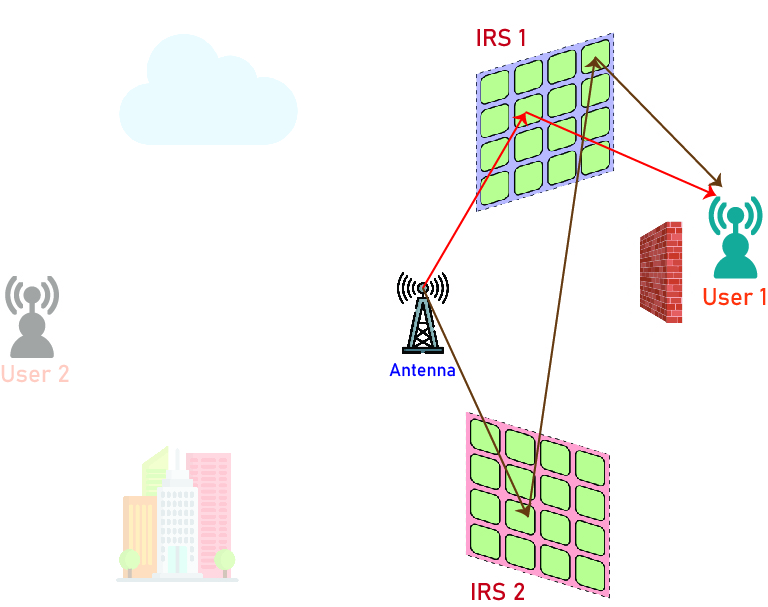
\includegraphics[scale=0.45]{with_obstacle__user1}
	
	\caption[سیگنال‌های دریافتی کاربر اول در شرایط با مانع]{
	سیگنال‌های دریافتی کاربر اول در شرایط با مانع
	}
%	\label{fig:fig-2_03}
\end{figure}

\begin{figure}[!h]
	\centering
	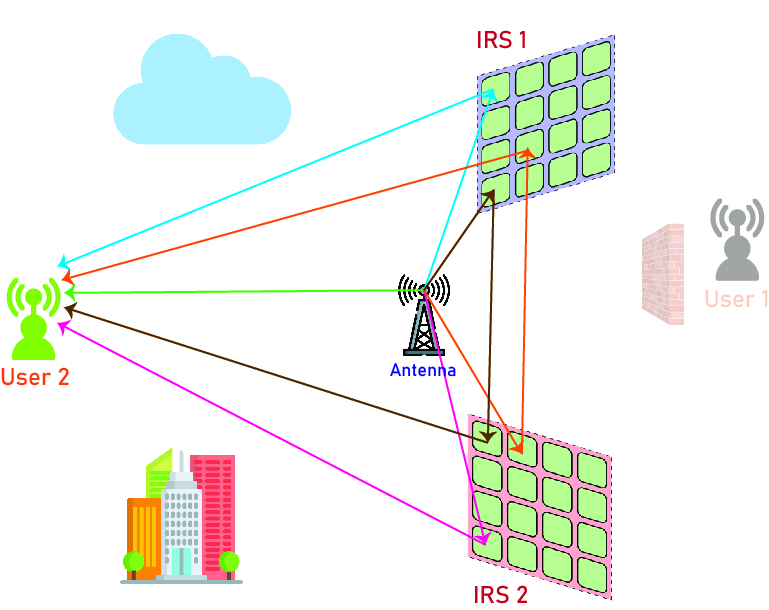
\includegraphics[scale=0.45]{with_obstacle__user2}
	
	\caption[سیگنال‌های دریافتی کاربر دوم در شرایط با مانع]{
		سیگنال‌های دریافتی کاربر دوم در شرایط با مانع
	}
%	\label{fig:fig-2_0}
\end{figure}
%%%%%%%%%%%%%%%%%%%%%%%%%%%%%%%%%%%%%%%%%%%
\newpage
\section{نوآوری ما}

در حال حاضر، همان‌طور که دیده‌اید، تعداد زیادی مقاله و مطلب در مورد مفهوم سطوح بازتابنده هوشمند وجود دارد. نه تنها تعداد اندکی از آن‌ها اثر بازتاب دوگانه یا بازتاب درجه دوم بین \lr{IRS} در کل عملکرد سیستم را در نظر گرفته‌اند، بلکه تقریباً تمامی آن‌ها اثر خط دید مستقیم (\lr{LoS}) را در این سناریوها با اعمال یک مانع نادیده گرفته‌اند. این نادیده‌گرفتن، انگیزه‌ای برای ما به وجود آورد تا یک سناریو را پیشنهاد دهیم تا اثر بازتاب دوگانه در حضور سیگنال‌های خط دید مستقیم را تجزیه و تحلیل کنیم. در این مقاله، به طور کلی، به تحلیل بهبودی که در حضور بازتاب دوگانه به دست می‌آید، می‌پردازیم تا ببینیم آیا اثر بازتاب دوگانه را می‌توان نادیده گرفت یا خیر.


\newpage
‌